% Options for packages loaded elsewhere
\PassOptionsToPackage{unicode}{hyperref}
\PassOptionsToPackage{hyphens}{url}
\PassOptionsToPackage{dvipsnames,svgnames,x11names}{xcolor}
%
\documentclass[
  letterpaper,
  DIV=11,
  numbers=noendperiod]{scrartcl}

\usepackage{amsmath,amssymb}
\usepackage{iftex}
\ifPDFTeX
  \usepackage[T1]{fontenc}
  \usepackage[utf8]{inputenc}
  \usepackage{textcomp} % provide euro and other symbols
\else % if luatex or xetex
  \usepackage{unicode-math}
  \defaultfontfeatures{Scale=MatchLowercase}
  \defaultfontfeatures[\rmfamily]{Ligatures=TeX,Scale=1}
\fi
\usepackage{lmodern}
\ifPDFTeX\else  
    % xetex/luatex font selection
\fi
% Use upquote if available, for straight quotes in verbatim environments
\IfFileExists{upquote.sty}{\usepackage{upquote}}{}
\IfFileExists{microtype.sty}{% use microtype if available
  \usepackage[]{microtype}
  \UseMicrotypeSet[protrusion]{basicmath} % disable protrusion for tt fonts
}{}
\makeatletter
\@ifundefined{KOMAClassName}{% if non-KOMA class
  \IfFileExists{parskip.sty}{%
    \usepackage{parskip}
  }{% else
    \setlength{\parindent}{0pt}
    \setlength{\parskip}{6pt plus 2pt minus 1pt}}
}{% if KOMA class
  \KOMAoptions{parskip=half}}
\makeatother
\usepackage{xcolor}
\setlength{\emergencystretch}{3em} % prevent overfull lines
\setcounter{secnumdepth}{-\maxdimen} % remove section numbering
% Make \paragraph and \subparagraph free-standing
\ifx\paragraph\undefined\else
  \let\oldparagraph\paragraph
  \renewcommand{\paragraph}[1]{\oldparagraph{#1}\mbox{}}
\fi
\ifx\subparagraph\undefined\else
  \let\oldsubparagraph\subparagraph
  \renewcommand{\subparagraph}[1]{\oldsubparagraph{#1}\mbox{}}
\fi

\usepackage{color}
\usepackage{fancyvrb}
\newcommand{\VerbBar}{|}
\newcommand{\VERB}{\Verb[commandchars=\\\{\}]}
\DefineVerbatimEnvironment{Highlighting}{Verbatim}{commandchars=\\\{\}}
% Add ',fontsize=\small' for more characters per line
\usepackage{framed}
\definecolor{shadecolor}{RGB}{241,243,245}
\newenvironment{Shaded}{\begin{snugshade}}{\end{snugshade}}
\newcommand{\AlertTok}[1]{\textcolor[rgb]{0.68,0.00,0.00}{#1}}
\newcommand{\AnnotationTok}[1]{\textcolor[rgb]{0.37,0.37,0.37}{#1}}
\newcommand{\AttributeTok}[1]{\textcolor[rgb]{0.40,0.45,0.13}{#1}}
\newcommand{\BaseNTok}[1]{\textcolor[rgb]{0.68,0.00,0.00}{#1}}
\newcommand{\BuiltInTok}[1]{\textcolor[rgb]{0.00,0.23,0.31}{#1}}
\newcommand{\CharTok}[1]{\textcolor[rgb]{0.13,0.47,0.30}{#1}}
\newcommand{\CommentTok}[1]{\textcolor[rgb]{0.37,0.37,0.37}{#1}}
\newcommand{\CommentVarTok}[1]{\textcolor[rgb]{0.37,0.37,0.37}{\textit{#1}}}
\newcommand{\ConstantTok}[1]{\textcolor[rgb]{0.56,0.35,0.01}{#1}}
\newcommand{\ControlFlowTok}[1]{\textcolor[rgb]{0.00,0.23,0.31}{#1}}
\newcommand{\DataTypeTok}[1]{\textcolor[rgb]{0.68,0.00,0.00}{#1}}
\newcommand{\DecValTok}[1]{\textcolor[rgb]{0.68,0.00,0.00}{#1}}
\newcommand{\DocumentationTok}[1]{\textcolor[rgb]{0.37,0.37,0.37}{\textit{#1}}}
\newcommand{\ErrorTok}[1]{\textcolor[rgb]{0.68,0.00,0.00}{#1}}
\newcommand{\ExtensionTok}[1]{\textcolor[rgb]{0.00,0.23,0.31}{#1}}
\newcommand{\FloatTok}[1]{\textcolor[rgb]{0.68,0.00,0.00}{#1}}
\newcommand{\FunctionTok}[1]{\textcolor[rgb]{0.28,0.35,0.67}{#1}}
\newcommand{\ImportTok}[1]{\textcolor[rgb]{0.00,0.46,0.62}{#1}}
\newcommand{\InformationTok}[1]{\textcolor[rgb]{0.37,0.37,0.37}{#1}}
\newcommand{\KeywordTok}[1]{\textcolor[rgb]{0.00,0.23,0.31}{#1}}
\newcommand{\NormalTok}[1]{\textcolor[rgb]{0.00,0.23,0.31}{#1}}
\newcommand{\OperatorTok}[1]{\textcolor[rgb]{0.37,0.37,0.37}{#1}}
\newcommand{\OtherTok}[1]{\textcolor[rgb]{0.00,0.23,0.31}{#1}}
\newcommand{\PreprocessorTok}[1]{\textcolor[rgb]{0.68,0.00,0.00}{#1}}
\newcommand{\RegionMarkerTok}[1]{\textcolor[rgb]{0.00,0.23,0.31}{#1}}
\newcommand{\SpecialCharTok}[1]{\textcolor[rgb]{0.37,0.37,0.37}{#1}}
\newcommand{\SpecialStringTok}[1]{\textcolor[rgb]{0.13,0.47,0.30}{#1}}
\newcommand{\StringTok}[1]{\textcolor[rgb]{0.13,0.47,0.30}{#1}}
\newcommand{\VariableTok}[1]{\textcolor[rgb]{0.07,0.07,0.07}{#1}}
\newcommand{\VerbatimStringTok}[1]{\textcolor[rgb]{0.13,0.47,0.30}{#1}}
\newcommand{\WarningTok}[1]{\textcolor[rgb]{0.37,0.37,0.37}{\textit{#1}}}

\providecommand{\tightlist}{%
  \setlength{\itemsep}{0pt}\setlength{\parskip}{0pt}}\usepackage{longtable,booktabs,array}
\usepackage{calc} % for calculating minipage widths
% Correct order of tables after \paragraph or \subparagraph
\usepackage{etoolbox}
\makeatletter
\patchcmd\longtable{\par}{\if@noskipsec\mbox{}\fi\par}{}{}
\makeatother
% Allow footnotes in longtable head/foot
\IfFileExists{footnotehyper.sty}{\usepackage{footnotehyper}}{\usepackage{footnote}}
\makesavenoteenv{longtable}
\usepackage{graphicx}
\makeatletter
\def\maxwidth{\ifdim\Gin@nat@width>\linewidth\linewidth\else\Gin@nat@width\fi}
\def\maxheight{\ifdim\Gin@nat@height>\textheight\textheight\else\Gin@nat@height\fi}
\makeatother
% Scale images if necessary, so that they will not overflow the page
% margins by default, and it is still possible to overwrite the defaults
% using explicit options in \includegraphics[width, height, ...]{}
\setkeys{Gin}{width=\maxwidth,height=\maxheight,keepaspectratio}
% Set default figure placement to htbp
\makeatletter
\def\fps@figure{htbp}
\makeatother

\KOMAoption{captions}{tableheading}
\makeatletter
\makeatother
\makeatletter
\makeatother
\makeatletter
\@ifpackageloaded{caption}{}{\usepackage{caption}}
\AtBeginDocument{%
\ifdefined\contentsname
  \renewcommand*\contentsname{Table of contents}
\else
  \newcommand\contentsname{Table of contents}
\fi
\ifdefined\listfigurename
  \renewcommand*\listfigurename{List of Figures}
\else
  \newcommand\listfigurename{List of Figures}
\fi
\ifdefined\listtablename
  \renewcommand*\listtablename{List of Tables}
\else
  \newcommand\listtablename{List of Tables}
\fi
\ifdefined\figurename
  \renewcommand*\figurename{Figure}
\else
  \newcommand\figurename{Figure}
\fi
\ifdefined\tablename
  \renewcommand*\tablename{Table}
\else
  \newcommand\tablename{Table}
\fi
}
\@ifpackageloaded{float}{}{\usepackage{float}}
\floatstyle{ruled}
\@ifundefined{c@chapter}{\newfloat{codelisting}{h}{lop}}{\newfloat{codelisting}{h}{lop}[chapter]}
\floatname{codelisting}{Listing}
\newcommand*\listoflistings{\listof{codelisting}{List of Listings}}
\makeatother
\makeatletter
\@ifpackageloaded{caption}{}{\usepackage{caption}}
\@ifpackageloaded{subcaption}{}{\usepackage{subcaption}}
\makeatother
\makeatletter
\@ifpackageloaded{tcolorbox}{}{\usepackage[skins,breakable]{tcolorbox}}
\makeatother
\makeatletter
\@ifundefined{shadecolor}{\definecolor{shadecolor}{rgb}{.97, .97, .97}}
\makeatother
\makeatletter
\makeatother
\makeatletter
\makeatother
\ifLuaTeX
  \usepackage{selnolig}  % disable illegal ligatures
\fi
\IfFileExists{bookmark.sty}{\usepackage{bookmark}}{\usepackage{hyperref}}
\IfFileExists{xurl.sty}{\usepackage{xurl}}{} % add URL line breaks if available
\urlstyle{same} % disable monospaced font for URLs
\hypersetup{
  colorlinks=true,
  linkcolor={blue},
  filecolor={Maroon},
  citecolor={Blue},
  urlcolor={Blue},
  pdfcreator={LaTeX via pandoc}}

\author{}
\date{}

\begin{document}
\ifdefined\Shaded\renewenvironment{Shaded}{\begin{tcolorbox}[interior hidden, breakable, frame hidden, sharp corners, enhanced, boxrule=0pt, borderline west={3pt}{0pt}{shadecolor}]}{\end{tcolorbox}}\fi


\includegraphics{./Титульник.jpeg} \textbf{Вариант 15}

\textbf{Цель работы:} изучить метод наименьших квадратов и применить его
на практике для получения коэффициентов линейной и квадратичной
функциональных зависсимостей.

\subsubsection{Входные
данные}\label{ux432ux445ux43eux434ux43dux44bux435-ux434ux430ux43dux43dux44bux435}

\begin{Shaded}
\begin{Highlighting}[]
\NormalTok{x }\OtherTok{\textless{}{-}} \FunctionTok{c}\NormalTok{(}\FloatTok{0.525}\NormalTok{, }\FloatTok{0.730}\NormalTok{, }\FloatTok{0.934}\NormalTok{, }\FloatTok{1.139}\NormalTok{, }\FloatTok{1.344}\NormalTok{, }\FloatTok{1.549}\NormalTok{, }\FloatTok{1.753}\NormalTok{, }\FloatTok{1.958}\NormalTok{, }\FloatTok{2.163}\NormalTok{, }\FloatTok{2.368}\NormalTok{)}
\NormalTok{y }\OtherTok{\textless{}{-}} \FunctionTok{c}\NormalTok{(}\FloatTok{0.360}\NormalTok{, }\FloatTok{0.426}\NormalTok{, }\FloatTok{0.483}\NormalTok{, }\FloatTok{0.561}\NormalTok{, }\FloatTok{0.610}\NormalTok{, }\FloatTok{0.645}\NormalTok{, }\FloatTok{0.710}\NormalTok{, }\FloatTok{0.737}\NormalTok{, }\FloatTok{0.736}\NormalTok{, }\FloatTok{0.773}\NormalTok{)}
\end{Highlighting}
\end{Shaded}

\paragraph{Код алгоритов Метода Гауса и нахождения
определителя}\label{ux43aux43eux434-ux430ux43bux433ux43eux440ux438ux442ux43eux432-ux43cux435ux442ux43eux434ux430-ux433ux430ux443ux441ux430-ux438-ux43dux430ux445ux43eux436ux434ux435ux43dux438ux44f-ux43eux43fux440ux435ux434ux435ux43bux438ux442ux435ux43bux44f}

\begin{Shaded}
\begin{Highlighting}[]
\NormalTok{gaussian\_elimination }\OtherTok{\textless{}{-}} \ControlFlowTok{function}\NormalTok{(A, b) \{}
\NormalTok{  n }\OtherTok{\textless{}{-}} \FunctionTok{nrow}\NormalTok{(A)}
  
\NormalTok{  Ab }\OtherTok{\textless{}{-}} \FunctionTok{cbind}\NormalTok{(A, b)}
  
  \CommentTok{\# Прямой ход}
  \ControlFlowTok{for}\NormalTok{ (i }\ControlFlowTok{in} \DecValTok{1}\SpecialCharTok{:}\NormalTok{(n }\SpecialCharTok{{-}} \DecValTok{1}\NormalTok{)) \{}
    \ControlFlowTok{if}\NormalTok{ (Ab[i, i] }\SpecialCharTok{==} \DecValTok{0}\NormalTok{) \{}
      \FunctionTok{message}\NormalTok{(}\StringTok{"Алгоритм не может продолжаться"}\NormalTok{)}
      \FunctionTok{return}\NormalTok{(}\ConstantTok{NULL}\NormalTok{)}
\NormalTok{    \}}
    
    \ControlFlowTok{for}\NormalTok{ (j }\ControlFlowTok{in}\NormalTok{ (i }\SpecialCharTok{+} \DecValTok{1}\NormalTok{)}\SpecialCharTok{:}\NormalTok{n) \{}
\NormalTok{      factor }\OtherTok{\textless{}{-}}\NormalTok{ Ab[j, i] }\SpecialCharTok{/}\NormalTok{ Ab[i, i]}
\NormalTok{      Ab[j, ] }\OtherTok{\textless{}{-}}\NormalTok{ Ab[j, ] }\SpecialCharTok{{-}}\NormalTok{ factor }\SpecialCharTok{*}\NormalTok{ Ab[i, ]}
\NormalTok{    \}}
\NormalTok{  \}}
  
  \CommentTok{\# Обратный ход}
\NormalTok{  x }\OtherTok{\textless{}{-}} \FunctionTok{numeric}\NormalTok{(n)}
\NormalTok{  x[n] }\OtherTok{\textless{}{-}}\NormalTok{ Ab[n, n }\SpecialCharTok{+} \DecValTok{1}\NormalTok{] }\SpecialCharTok{/}\NormalTok{ Ab[n, n]}
  
  \ControlFlowTok{for}\NormalTok{ (i }\ControlFlowTok{in}\NormalTok{ (n }\SpecialCharTok{{-}} \DecValTok{1}\NormalTok{)}\SpecialCharTok{:}\DecValTok{1}\NormalTok{) \{}
\NormalTok{    x[i] }\OtherTok{\textless{}{-}}\NormalTok{ (Ab[i, n }\SpecialCharTok{+} \DecValTok{1}\NormalTok{] }\SpecialCharTok{{-}} \FunctionTok{sum}\NormalTok{(Ab[i, (i }\SpecialCharTok{+} \DecValTok{1}\NormalTok{)}\SpecialCharTok{:}\NormalTok{n] }\SpecialCharTok{*}\NormalTok{ x[(i }\SpecialCharTok{+} \DecValTok{1}\NormalTok{)}\SpecialCharTok{:}\NormalTok{n])) }\SpecialCharTok{/}\NormalTok{ Ab[i, i]}
\NormalTok{  \}}
  
  \FunctionTok{return}\NormalTok{(x)}
\NormalTok{\}}
\end{Highlighting}
\end{Shaded}

\begin{Shaded}
\begin{Highlighting}[]
\NormalTok{determinant }\OtherTok{\textless{}{-}} \ControlFlowTok{function}\NormalTok{(matrix) \{}
  \ControlFlowTok{if}\NormalTok{ (}\FunctionTok{ncol}\NormalTok{(matrix) }\SpecialCharTok{==} \FunctionTok{nrow}\NormalTok{(matrix)) \{}
    \ControlFlowTok{if}\NormalTok{ (}\FunctionTok{ncol}\NormalTok{(matrix) }\SpecialCharTok{==} \DecValTok{1}\NormalTok{) \{}
      \FunctionTok{return}\NormalTok{(matrix[}\DecValTok{1}\NormalTok{, }\DecValTok{1}\NormalTok{])}
\NormalTok{    \} }\ControlFlowTok{else} \ControlFlowTok{if}\NormalTok{ (}\FunctionTok{ncol}\NormalTok{(matrix) }\SpecialCharTok{==} \DecValTok{2}\NormalTok{) \{}
\NormalTok{      result }\OtherTok{\textless{}{-}}\NormalTok{ (matrix[}\DecValTok{1}\NormalTok{, }\DecValTok{1}\NormalTok{] }\SpecialCharTok{*}\NormalTok{ matrix[}\DecValTok{2}\NormalTok{, }\DecValTok{2}\NormalTok{]) }\SpecialCharTok{{-}}\NormalTok{ (matrix[}\DecValTok{1}\NormalTok{, }\DecValTok{2}\NormalTok{] }\SpecialCharTok{*}\NormalTok{ matrix[}\DecValTok{2}\NormalTok{, }\DecValTok{1}\NormalTok{])}
      \FunctionTok{return}\NormalTok{(result)}
\NormalTok{    \} }\ControlFlowTok{else}\NormalTok{ \{}
\NormalTok{      det }\OtherTok{\textless{}{-}} \DecValTok{0}
      \ControlFlowTok{for}\NormalTok{ (i }\ControlFlowTok{in} \DecValTok{1}\SpecialCharTok{:}\FunctionTok{ncol}\NormalTok{(matrix)) \{}
\NormalTok{        sign }\OtherTok{\textless{}{-}}\NormalTok{ (}\SpecialCharTok{{-}}\DecValTok{1}\NormalTok{)}\SpecialCharTok{\^{}}\NormalTok{(i}\SpecialCharTok{+}\DecValTok{1}\NormalTok{)}
\NormalTok{        minor }\OtherTok{\textless{}{-}}\NormalTok{ matrix[}\SpecialCharTok{{-}}\DecValTok{1}\NormalTok{, }\SpecialCharTok{{-}}\NormalTok{i]}
\NormalTok{        det }\OtherTok{\textless{}{-}}\NormalTok{ det }\SpecialCharTok{+}\NormalTok{ sign }\SpecialCharTok{*}\NormalTok{ matrix[}\DecValTok{1}\NormalTok{, i] }\SpecialCharTok{*} \FunctionTok{determinant}\NormalTok{(minor)}
\NormalTok{      \}}
      \FunctionTok{return}\NormalTok{(det)}
\NormalTok{    \}}
\NormalTok{  \} }\ControlFlowTok{else}\NormalTok{ \{}
    \FunctionTok{return}\NormalTok{(}\StringTok{"Матрица не квадратная"}\NormalTok{)}
\NormalTok{  \}}
\NormalTok{\}}
\end{Highlighting}
\end{Shaded}

\begin{figure}

{\centering 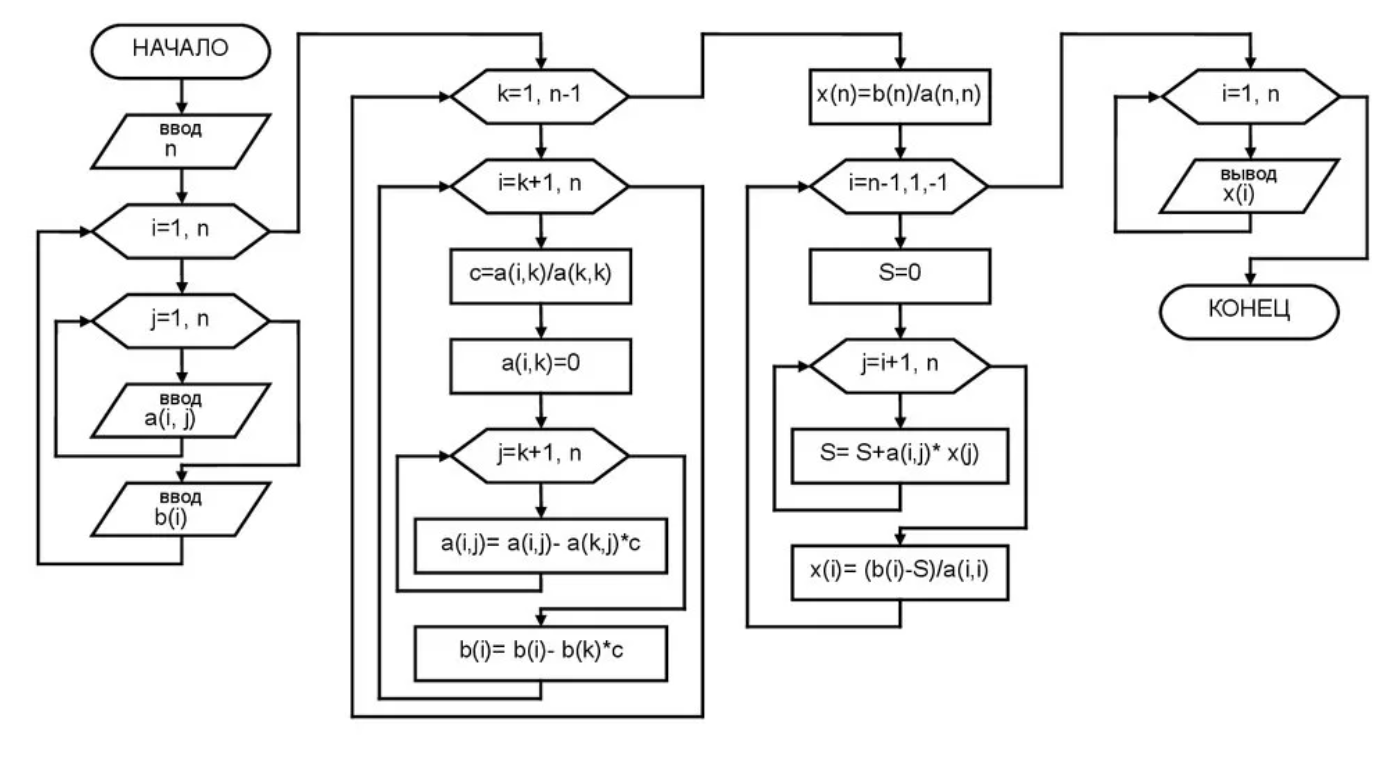
\includegraphics{./Gaus.png}

}

\caption{\label{fig-gaus}Блок-схема алгоритма Метода Гауса}

\end{figure}

\subsubsection{Для линейной апроксимирующей
функции}\label{ux434ux43bux44f-ux43bux438ux43dux435ux439ux43dux43eux439-ux430ux43fux440ux43eux43aux441ux438ux43cux438ux440ux443ux44eux449ux435ux439-ux444ux443ux43dux43aux446ux438ux438}

\paragraph{Система линейных алгебраических
уравнений}\label{ux441ux438ux441ux442ux435ux43cux430-ux43bux438ux43dux435ux439ux43dux44bux445-ux430ux43bux433ux435ux431ux440ux430ux438ux447ux435ux441ux43aux438ux445-ux443ux440ux430ux432ux43dux435ux43dux438ux439}

\[y_i = a x_i + b + \delta_i\]

\[
\begin{cases}
a \sum_{i=1}^n x_i^2 + b \sum_{i=1}^n x_i = \sum_{i=1}^n x_i y_i \\ \\
a \sum_{i=1}^n x_i + b n = \sum_{i=1}^n y_i
\end{cases}
\]

\begin{figure}

{\centering 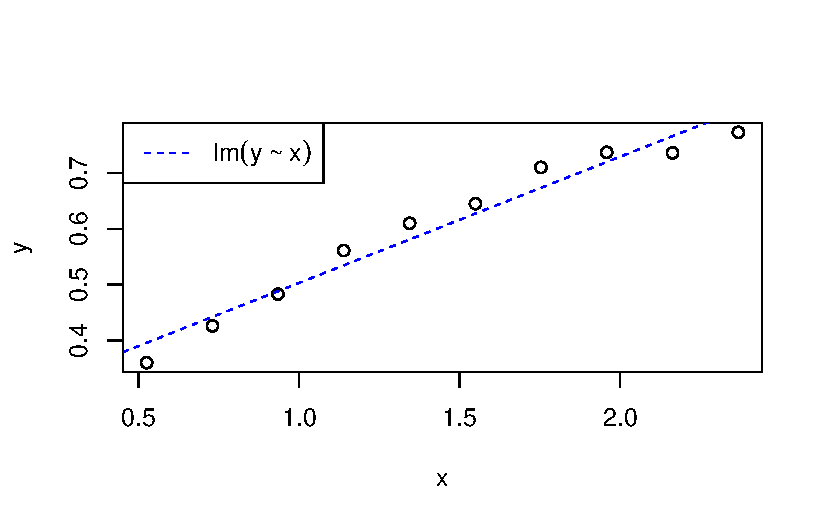
\includegraphics{main_files/figure-pdf/fig-lin-aprox-builtin-1.pdf}

}

\caption{\label{fig-lin-aprox-builtin}График встроенной линейной
апроксимирующей функции}

\end{figure}

\paragraph{Получение
значений}\label{ux43fux43eux43bux443ux447ux435ux43dux438ux435-ux437ux43dux430ux447ux435ux43dux438ux439}

\begin{Shaded}
\begin{Highlighting}[]
\NormalTok{k11 }\OtherTok{\textless{}{-}} \FunctionTok{sum}\NormalTok{(x}\SpecialCharTok{\^{}}\DecValTok{2}\NormalTok{)}
\NormalTok{k12 }\OtherTok{\textless{}{-}} \FunctionTok{sum}\NormalTok{(x)}
\NormalTok{b1  }\OtherTok{\textless{}{-}} \FunctionTok{sum}\NormalTok{(x }\SpecialCharTok{*}\NormalTok{ y)}

\NormalTok{k21 }\OtherTok{\textless{}{-}} \FunctionTok{sum}\NormalTok{(x)}
\NormalTok{k22 }\OtherTok{\textless{}{-}} \FunctionTok{length}\NormalTok{(x)}
\NormalTok{b2  }\OtherTok{\textless{}{-}} \FunctionTok{sum}\NormalTok{(y)}

\NormalTok{m1 }\OtherTok{\textless{}{-}} \FunctionTok{matrix}\NormalTok{(}\FunctionTok{c}\NormalTok{(k11, k12,}
\NormalTok{               k21, k22), }\AttributeTok{ncol=}\DecValTok{2}\NormalTok{, }\AttributeTok{byrow=}\NormalTok{T)}


\NormalTok{m1\_a }\OtherTok{=} \FunctionTok{matrix}\NormalTok{(}\FunctionTok{c}\NormalTok{(b1, k12,}
\NormalTok{                b2, k22), }\AttributeTok{ncol=}\DecValTok{2}\NormalTok{, }\AttributeTok{byrow=}\NormalTok{T)}

\NormalTok{m1\_b }\OtherTok{=} \FunctionTok{matrix}\NormalTok{(}\FunctionTok{c}\NormalTok{(k11, b1,}
\NormalTok{                k21, b2), }\AttributeTok{ncol=}\DecValTok{2}\NormalTok{, }\AttributeTok{byrow=}\NormalTok{T)}

\NormalTok{det\_m1 }\OtherTok{\textless{}{-}} \FunctionTok{determinant}\NormalTok{(m1)}
\NormalTok{det\_a }\OtherTok{=} \FunctionTok{determinant}\NormalTok{(m1\_a)}
\NormalTok{det\_b }\OtherTok{=} \FunctionTok{determinant}\NormalTok{(m1\_b)}

\NormalTok{a }\OtherTok{=}\NormalTok{ det\_a }\SpecialCharTok{/}\NormalTok{ det\_m1}
\NormalTok{b }\OtherTok{=}\NormalTok{ det\_b }\SpecialCharTok{/}\NormalTok{ det\_m1}

\NormalTok{a\_accurate }\OtherTok{\textless{}{-}} \FunctionTok{coef}\NormalTok{(f1)[}\DecValTok{2}\NormalTok{]}
\NormalTok{b\_accurate }\OtherTok{\textless{}{-}} \FunctionTok{coef}\NormalTok{(f1)[}\DecValTok{1}\NormalTok{]}

\NormalTok{a\_abs\_err }\OtherTok{\textless{}{-}} \FunctionTok{abs}\NormalTok{(a\_accurate }\SpecialCharTok{{-}}\NormalTok{ a)}
\NormalTok{b\_abs\_err }\OtherTok{\textless{}{-}} \FunctionTok{abs}\NormalTok{(b\_accurate }\SpecialCharTok{{-}}\NormalTok{ b)}
\NormalTok{a\_rel\_err }\OtherTok{\textless{}{-}}\NormalTok{ a\_abs\_err }\SpecialCharTok{/} \FunctionTok{abs}\NormalTok{(a\_accurate)}
\NormalTok{b\_rel\_err }\OtherTok{\textless{}{-}}\NormalTok{ b\_abs\_err }\SpecialCharTok{/} \FunctionTok{abs}\NormalTok{(b\_accurate)}
\end{Highlighting}
\end{Shaded}

\(a_{точн.} = 0.2260958 \quad a_{получ.} = 0.2260958\)\\
\(b_{точн.} = 0.2770976 \quad b_{получ.} = 0.2770976\)

\(\Delta a = \ensuremath{8.3266727\times 10^{-17}} \quad \delta a = \ensuremath{3.6828066\times 10^{-16}}\)\\
\(\Delta b = \ensuremath{7.2164497\times 10^{-16}} \quad \delta b = \ensuremath{2.604299\times 10^{-15}}\)

\begin{figure}

{\centering 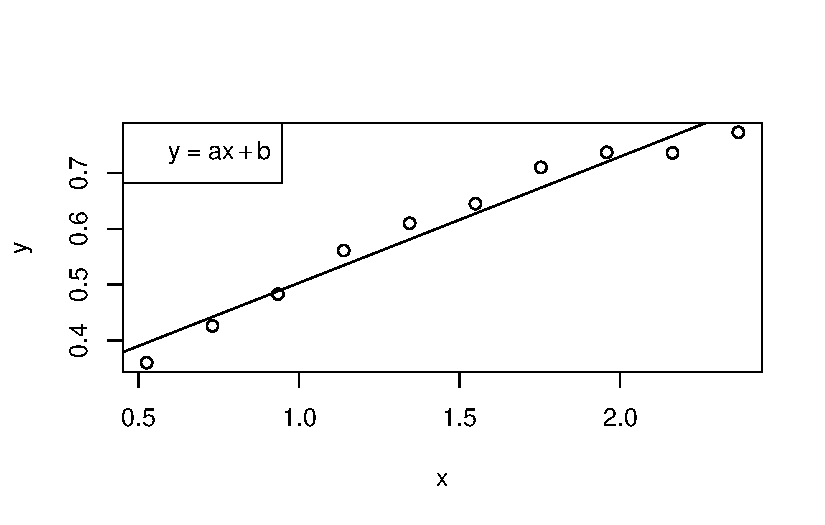
\includegraphics{main_files/figure-pdf/fig-lin-approx-my-1.pdf}

}

\caption{\label{fig-lin-approx-my}График полученной линейной
апроксимирующей функции}

\end{figure}

\subsubsection{Для квадратичной апроксимирующей
функции}\label{ux434ux43bux44f-ux43aux432ux430ux434ux440ux430ux442ux438ux447ux43dux43eux439-ux430ux43fux440ux43eux43aux441ux438ux43cux438ux440ux443ux44eux449ux435ux439-ux444ux443ux43dux43aux446ux438ux438}

\paragraph{Система линейных алгебраических
уравнений}\label{ux441ux438ux441ux442ux435ux43cux430-ux43bux438ux43dux435ux439ux43dux44bux445-ux430ux43bux433ux435ux431ux440ux430ux438ux447ux435ux441ux43aux438ux445-ux443ux440ux430ux432ux43dux435ux43dux438ux439-1}

\[
y_i = a_0 + a_1 x_1 + a_2 x_i^2 + \delta_i
\]

\[
\begin{cases}
a_0 \sum_{i=1}^n x_i^2 + a_1 \sum_{i=1}^n x_i + a_2 n = \sum_{i=1}^n y_i \\ \\
a_0 \sum_{i=1}^n x_i^2 + a_1 \sum_{i=1}^n x_i^2 + a_2 x_i = \sum_{i=1}^n x_iy_i \\ \\
a_0 \sum_{i=1}^n x^4 + a_1 \sum_{i=1}^n x_i^2 + a_2 \sum_{i=1}^n = x_i^2y_i
\end{cases}
\]

\paragraph{Точные
коэффициенты}\label{ux442ux43eux447ux43dux44bux435-ux43aux43eux44dux444ux444ux438ux446ux438ux435ux43dux442ux44b}

\begin{Shaded}
\begin{Highlighting}[]
\NormalTok{as\_accurate }\OtherTok{\textless{}{-}} \FunctionTok{c}\NormalTok{(}\FloatTok{0.120}\NormalTok{, }\FloatTok{0.486}\NormalTok{, }\SpecialCharTok{{-}}\FloatTok{0.090}\NormalTok{)}
\end{Highlighting}
\end{Shaded}

\begin{figure}

{\centering 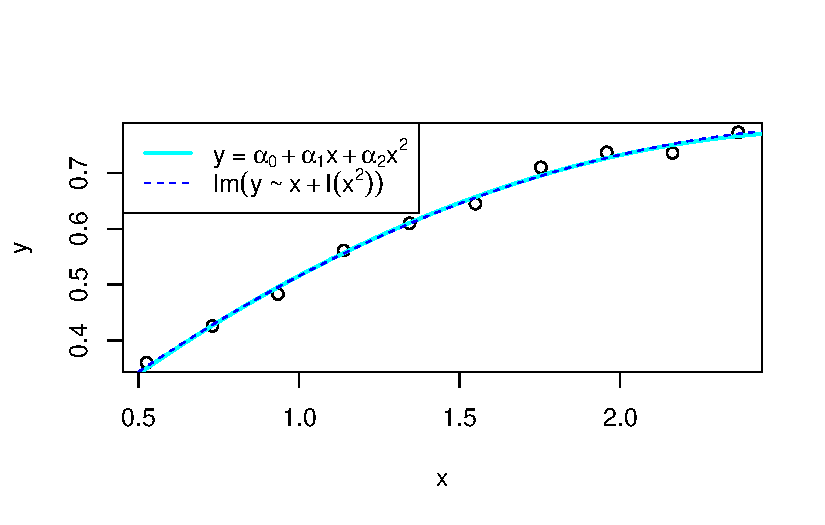
\includegraphics{main_files/figure-pdf/fig-square-approx-defined-1.pdf}

}

\caption{\label{fig-square-approx-defined}График точной и встроенной
квадратичной апроксимирующей функции}

\end{figure}

\paragraph{Получение
значений}\label{ux43fux43eux43bux443ux447ux435ux43dux438ux435-ux437ux43dux430ux447ux435ux43dux438ux439-1}

\begin{Shaded}
\begin{Highlighting}[]
\NormalTok{k11 }\OtherTok{\textless{}{-}} \FunctionTok{sum}\NormalTok{(x}\SpecialCharTok{\^{}}\DecValTok{2}\NormalTok{)}
\NormalTok{k12 }\OtherTok{\textless{}{-}} \FunctionTok{sum}\NormalTok{(x)}
\NormalTok{k13 }\OtherTok{\textless{}{-}} \FunctionTok{length}\NormalTok{(x)}
\NormalTok{b1  }\OtherTok{\textless{}{-}} \FunctionTok{sum}\NormalTok{(y)}

\NormalTok{k21 }\OtherTok{\textless{}{-}} \FunctionTok{sum}\NormalTok{(x}\SpecialCharTok{\^{}}\DecValTok{3}\NormalTok{)}
\NormalTok{k22 }\OtherTok{\textless{}{-}} \FunctionTok{sum}\NormalTok{(x}\SpecialCharTok{\^{}}\DecValTok{2}\NormalTok{)}
\NormalTok{k23 }\OtherTok{\textless{}{-}} \FunctionTok{sum}\NormalTok{(x)}
\NormalTok{b2  }\OtherTok{\textless{}{-}} \FunctionTok{sum}\NormalTok{(x}\SpecialCharTok{*}\NormalTok{y)}

\NormalTok{k31 }\OtherTok{\textless{}{-}} \FunctionTok{sum}\NormalTok{(x}\SpecialCharTok{\^{}}\DecValTok{4}\NormalTok{)}
\NormalTok{k32 }\OtherTok{\textless{}{-}} \FunctionTok{sum}\NormalTok{(x}\SpecialCharTok{\^{}}\DecValTok{3}\NormalTok{)}
\NormalTok{k33 }\OtherTok{\textless{}{-}} \FunctionTok{sum}\NormalTok{(x}\SpecialCharTok{\^{}}\DecValTok{2}\NormalTok{)}
\NormalTok{b3  }\OtherTok{\textless{}{-}} \FunctionTok{sum}\NormalTok{(x}\SpecialCharTok{\^{}}\DecValTok{2} \SpecialCharTok{*}\NormalTok{ y)}

\NormalTok{bs    }\OtherTok{\textless{}{-}} \FunctionTok{c}\NormalTok{(b1, b2, b3)}

\NormalTok{m2    }\OtherTok{\textless{}{-}} \FunctionTok{matrix}\NormalTok{(}\FunctionTok{c}\NormalTok{(k11, k12, k13,}
\NormalTok{                  k21, k22, k23,}
\NormalTok{                  k31, k32, k33), }\AttributeTok{ncol=}\DecValTok{3}\NormalTok{, }\AttributeTok{nrow=}\DecValTok{3}\NormalTok{, }\AttributeTok{byrow=}\NormalTok{T)}

\NormalTok{as\_my }\OtherTok{\textless{}{-}} \FunctionTok{rev}\NormalTok{(}\FunctionTok{gaussian\_elimination}\NormalTok{(m2, bs))}

\NormalTok{res\_solve }\OtherTok{\textless{}{-}} \FunctionTok{solve}\NormalTok{(m2, bs)}

\NormalTok{as\_abs\_err }\OtherTok{=} \FunctionTok{abs}\NormalTok{(as\_accurate }\SpecialCharTok{{-}}\NormalTok{ as\_my)}
\NormalTok{as\_rel\_err }\OtherTok{=}\NormalTok{ as\_abs\_err }\SpecialCharTok{/} \FunctionTok{abs}\NormalTok{(as\_my)}
\end{Highlighting}
\end{Shaded}

\(\alpha_{точн.} = (0.12, 0.486, -0.09)^T\)\\
\(a_{получ.} = (0.1300611, 0.4696716, -0.084198)^T\)

\(\Delta a = ( 0.0100611, 0.0163284, 0.005802)^T\)\\
\(\delta a = (0.0773566, 0.0347657, 0.0689086)^T\)

\begin{figure}

{\centering 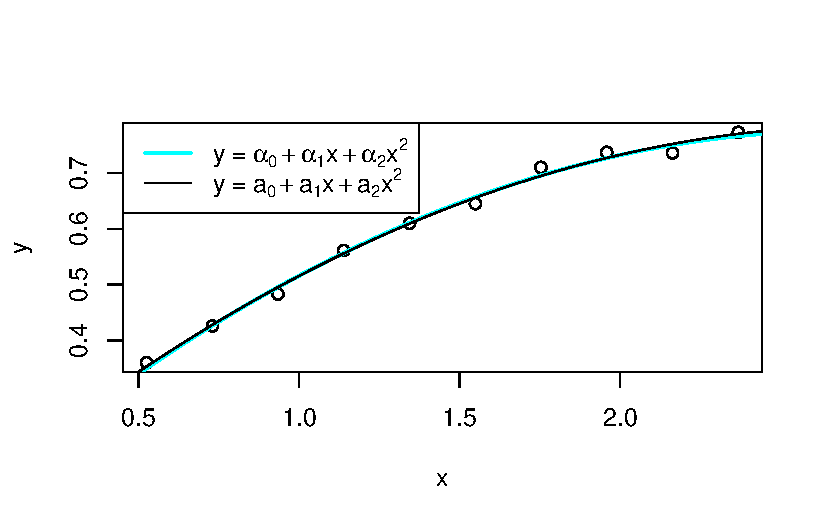
\includegraphics{main_files/figure-pdf/fig-square-approx-my-1.pdf}

}

\caption{\label{fig-square-approx-my}График точной и полученной
квадратичной апроксимирующей функции}

\end{figure}

\subsubsection{Вывод}\label{ux432ux44bux432ux43eux434}

Были получены коэффициенты линейной и квадратичной зависсимостей методом
Краммера и Гауса, построены графики функций, посчитаны погрешности.
Графики, построенные по найденным коэффициентам, совпали с ожидаемыми в
рамках погрешности.



\end{document}
